\chapter{Bruits et parasites}
Introduisons la notion de  bruit et parasite:
\begin{description}
	\item[Bruit] au sens strict (encore appelé "bruit de fond") est un signal à variation aléatoire d'origine \emph{interne} au dispositif étudié. Il est possible de le définir, de prévoir son niveau plancher à l'aide du dimensionnement
	\item[Parasites] signaux perturbateurs d'origine \emph{externe} au dispositif
\end{description}
Ces 2 phénomènes se présentent sous forme de signal analogique venant s'additionner au signal utile, entraînant ainsi sa dégradation. Une fois le signal utile perturbé, pas de marche arrière, d'où l'importance des ces concepts lors du dimensionnement.
\begin{table}[H]
	\centering
	\begin{tabular}{lcr}
		& \textbf{bruit} & \textbf{parasite} \\ \hline
		origine & interne & externe \\
		distribution & aléatoire & variable \\
		bande passante & "\(\infty\)" & limitée \\
		amplitude & faible & variable \\
		& "plancher" & arbitrairement bas \\
		modélisation & "facile" & difficile \\
		contre-mesures & conception & conception/remédiation \\ \hline
 	\end{tabular}
	\caption{Critères de distinction}
\end{table}
On remarque que:
\begin{itemize}
	\item contrairement au bruit qui possède généralement une amplitude plancher, calculable théoriquement, il est théoriquement impossible de réduire les parasites à un niveau arbitrairement bas.
	\item La modélisation des effets du bruit dans un système est, dans le principe, simple. Au contraire, la modélisation des parasites est nettement plus difficile car ceux-ci sont constitués de plusieurs signaux plus déterministes dont il faut connaître les couplages avec le système étudié.
\end{itemize}
L'introduction des ces phénomènes relève tout l'intérêt des signaux numérique (au lieu d'analogique). En effet, alors qu'un signal analogique dégradé ne peut être restauré, il est possible généralement de restaurer un signal numérique dégradé.\\
Un signal numérique n'est rien d'autre qu'un signal analogique dont certains niveaux représentent des valeurs discrètes portant une information (paliers, ex. 0=vrai, 1=faux) et dont chaque niveau peut varier dans certaines limite \(\rightarrow\) marges de bruit.\\

Ainsi, si l'impact des bruits et parasites est inférieur à cette marge de bruit définie par la conception, il est possible de restaurer le signal numérique utile. Les signaux numériques présentent donc une meilleure robustesse face aux perturbations. Il sera néanmoins toujours nécessaire de limiter les perturbations (car marges de bruit limitées).
\section{Le bruit de fond}
\subsection{Introduction}
Le bruit de fond possède plusieurs caractéristiques:
\begin{itemize}
	\item fluctuation aléatoire fondamentale due à la nature elle-même du dispositif
	\item limite ultime de la résolution du dispositif (contrairement aux parasites)
	\item fondamentalement inévitable (jamais nul) mais son influence sur la chaîne peut être minimisée
	\item origine générale en électronique: fluctuations de la densité des porteurs de charges (porteurs de charges = \(e^-\) et trous, fonction de la température)
	\item observable sur une tension et/ou un courant
\end{itemize}
Il existe plusieurs type de bruit, comme le bruit de type gaussien (c-à-d qui suit une loi normale de moyenne et variance données \(N(\mu,\sigma)\), \autoref{fig:densiteprobagauss})

\begin{figure}[H] 
	\centering 
\pgfmathdeclarefunction{gauss}{2}{%
	\pgfmathparse{1/(#2*sqrt(2*pi))*exp(-((x-#1)^2)/(2*#2^2))}%
}
	\begin{tikzpicture}[
	scale=0.6,
	every pin edge/.style={<-},
	every pin/.style={fill=yellow!50,rectangle,rounded corners=3pt,font=\small}]
	\begin{axis}[every axis plot post/.append style={
		mark=none,domain=-3:3,samples=30,smooth},
	clip=false,
	axis y line=none,
	axis x line*=bottom,
	ymin=0,
	xtick=\empty,
	]
	\addplot {gauss(0,0.5)};
	\addplot {gauss(0,1)};
	\draw[dashed]  (axis description cs:0.5,0) node[below] {\(\mu\)} -- (axis description cs:0.5,0.92) ;
	\end{axis}
	\end{tikzpicture}
\caption{Bruit de type gaussien: densité de probabilité}
\label{fig:densiteprobagauss}
\end{figure}
Valeur maximale du bruit ? Prenons un bruit de valeur efficace \(\SI{1}{\volt}\) (\autoref{fig:tensionbruitmax}). Il est tout à fait possible qu'au bout de \(\SI{100}{\second}\) on ait un bruit 10 fois plus grand. C'est aléatoire, mais sa puissance rms est constante.
\begin{figure}[H] 
	\centering 
	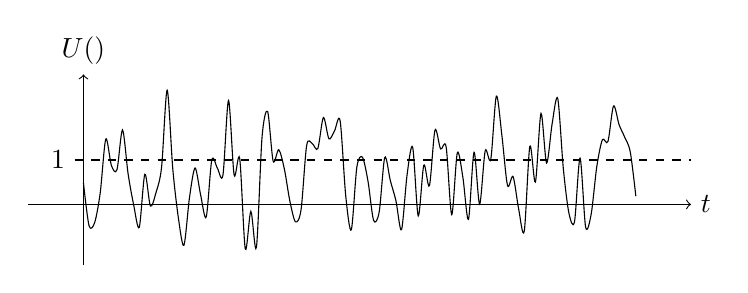
\begin{tikzpicture}[samples=100, domain=0:5*360]
	\begin{axis}[
	width=10cm, height=4cm,
	enlarge x limits=true,
	xtick=\empty,
	ytick=\empty,
	axis line style={->},
	axis lines*=middle,
	xlabel=\(t\),
	ylabel=\(U(\si{\volt})\),
	every axis x label/.style={
		at={(ticklabel* cs:1)},
		anchor=west,
	},
	every axis y label/.style={
		at={(ticklabel* cs:1)},
		anchor=south,
	},]
	\addplot [no markers, smooth] {sin(x)*sin(x)+rand};
	\draw[dashed] (axis description cs:0.07,0.55) node[left] {\SI{1}{\volt}} -- (axis description cs:1,0.55) ;
		\end{axis}
	\end{tikzpicture}
	\caption{Bruit de type gaussien: tension} 
	\label{fig:tensionbruitmax}
\end{figure}

\paragraph{Remarque:} la "valeur efficace" est une puissance mesurée, ce n'est pas le max
\subsection{Caractérisation mathématique}
\subsubsection{Définition de base}
Mathématiquement, le bruit est caractérisé par un \emph{signal temporel} (f.e.m) \(E_b(t)\) avec les propriétés suivantes:
\begin{itemize}
	\item {\makebox[8cm]{fluctuation aléatoire \(\Rightarrow\) moyenne nulle\hfill} \(\overline{E_b(t)}=0\)}
	\item {\makebox[8cm]{valeur quadratique moyenne non nulle\hfill} \(\overline{E_b^2(t)} \neq 0\)}
	\item {\makebox[8cm]{valeur efficace ("rms" = root mean square)\hfill} \(E_b=\sqrt{\overline{E_b^2(t)}}\)}
	\item {\makebox[8cm]{rapport signal/bruit SNR [dB]\hfill} \(SNR=10\log\left(\overline{E^2_s(t)}/\overline{E_b^2(t)}\right)\)}
\end{itemize}
\subsubsection{Variation en fréquence}
À ces propriétés s'ajoutent:\begin{itemize}
	\item La valeur efficace dépend de la fréquence \(\Rightarrow\) \emph{densité spectrale} de bruit \[e_b(f)=\sqrt{\left.\frac{d\overline{E_b^2}}{df}\right|_f}\quad [\si[per-mode=symbol]{\volt\per\sqrt{\hertz}}]\]
	\item La couleur du bruit:
	\begin{itemize}
		\item bruit blanc: densité spectrale constante en fréquence (uniformément réparti en fréquence, \autoref{fig:bruitblanc})
		\item bruit rose: densité spectrale plus forte pour les basses fréquences (descente linéaire, \autoref{fig:bruitrose})
	\end{itemize}
\end{itemize}
\begin{figure}[H]
	\centering
	\subfigure[Bruit blanc]{\label{fig:bruitblanc}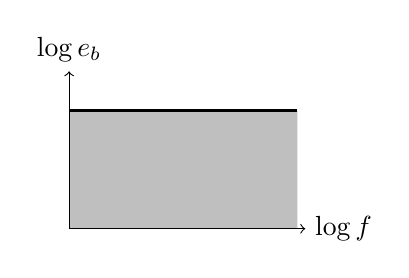
\begin{tikzpicture}
		\fill [gray!50, domain=0:2.9, variable=\x]
		(0, 0)
		-- plot ({\x}, {1.5})
		-- (2.9, 0)
		-- cycle;
		\draw[->] (0,0) -- (0,2) node[above]{\(\log e_b\)};
		\draw[->] (0,0) -- (3,0) node[right]{\(\log f\)};
		\draw[very thick] (0,1.5) -- (2.9,1.5);
		\end{tikzpicture}}
	\subfigure[Bruit rose]{\label{fig:bruitrose}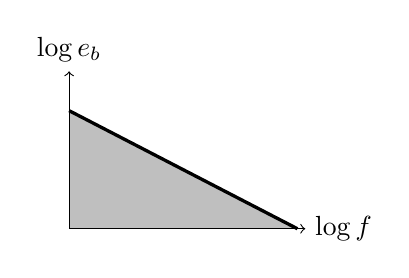
\begin{tikzpicture}
		\fill [gray!50, domain=0:2.9, variable=\x]
		(0, 0)
		-- plot ({\x}, {1.5-\x*0.51})
		-- (2.9, 0)
		-- cycle;
		\draw[->] (0,0) -- (0,2) node[above]{\(\log e_b\)};
		\draw[->] (0,0) -- (3,0) node[right]{\(\log f\)};
		\draw[very thick] (0,1.5) -- (2.9,0);
		\end{tikzpicture}}
	\caption{Répartition en fréquence de la densité spectrale de bruit}
\end{figure}
\subsubsection{Sommation de bruits divers}
Dans l'hypothèse où il n'y a pas corrélation entre:
\begin{itemize}
	\item les sources de bruits d'origine différente
	\item la même source à différentes fréquences
\end{itemize}
\centerline{\(\Rightarrow\) Puissance totale de bruit = \(\sum\) des puissance de bruit individuelles.}
Or la puissance de bruit \(\propto\) valeur quadratique moyenne de la tension ou du courant de bruit \(\rightarrow P_b=R \overline{I^2_b} = \frac{\overline{V_b^2}}{R}\). Il faut donc sommer \emph{quadratiquement} tensions et courants de bruit 
\[
V_b^2 = V_{b_1}^2 + V_{b_2}^2 + \dots + V_{b_n}^2 \qquad I_b^2 = I_{b_1}^2 + I_{b_2}^2 + \dots + I_{b_n}^2
\]
De même pour les densités spectrales:
\[
v_b^2(f) = v_{b_1}^2(f) + v_{b_2}^2(f) + \dots + v_{b_n}^2(f)
\]
\subsection{Types de bruit}
\subsubsection{Bruit thermique ou de Johnson}
Le bruit thermique est un bruit dû à l'agitation thermique des porteurs de charges (\(e^-\) dans conducteur, \(e^-+\) trous dans semi-conducteur). À \(T>\SI{0}{\kelvin}\), il y a collision des porteurs de charges entre eux \(\rightarrow\) répartition non uniforme des charges électriques \(\rightarrow\) champ électrique variable aléatoirement.\bigbreak

Ses propriétés sont les suivantes:
\begin{itemize}
	\item {\makebox[6cm]{valeur moyenne nulle\hfill} \(\overline{E_{bR}(t)}=0\)} 
	\item {\makebox[6cm]{valeur quadratique moyenne\hfill} \(\overline{E^2_{bR}(t)}=4kRT\Delta f\)} avec \(\left\{\substack{k\text{ : cst de Boltzmann }=\SI[per-mode=symbol]{1.374e-23}{\joule\per\kelvin}\\
	R \text{ : résistance en }\si{\ohm}\hfill \\
	T\text{ : température absolue en }\si{\kelvin}\hfill\\
	\Delta f\text{ : bande de fréquence observée}\hfill}\right.\)
	\item bruit blanc
	\item existe dans toute résistance vraie
	\item mesurable malgré son faible ordre de grandeur\footnote{Potentiel du cerveau \(\approx \SI{1}{\micro\volt}\)}
\end{itemize}
\subsubsection{Bruits en 1/f}
Les bruits en 1/f sont plus fort à basses qu'à hautes fréquences (bruit rose), il en existe 2 types:
\begin{itemize}
	\item Bruit de scintillation:
	\begin{itemize}
		\item présent dans les semi-conducteurs
		\item d'origine incertaine, recombinaisons dans les défauts de surface du semi-conducteur (\(e^-\) et trous)
	\end{itemize}
	\item Bruit en excès (ou bruit de constitution, "contact noise", "excess noise"):
	\begin{itemize}
		\item analogue au bruit de scintillation
		\item présent dans certaines résistances (ex. résistance à couche de carbones)
		\item engendré par l'évolution erratique (:= aléatoire) des lignes de courant (continu) dans un matériau non homogène
	\end{itemize}
\end{itemize}
\subsubsection{Autres types de bruit}
Le reste:
\begin{itemize}
	\item Bruit de grenaille (ou de Schottky):
	\begin{itemize}
		\item présent dans les semi-conducteurs
		\item dû à la nature quantifié du courant électrique, provoqué par passage des porteurs de charge au travers d'une barrière de potentiel
	\end{itemize}
	\item Bruit quantique:
	\begin{itemize}
		\item dû à la nature quantifiée de l'énergie rayonnée (photons)
	\end{itemize}
	\item Bruit de diffusion:
	\begin{itemize}
		\item présent dans les semi-conducteurs
		\item dû aux collisions des porteurs de charges avec le réseau cristallin
	\end{itemize}
	\item Bruit de génération/recombinaison:
	\begin{itemize}
		\item présent dans les semi-conducteurs
		\item  dû à la fluctuation aléatoire des taux de génération, des recombinaisons et des piégeages des porteurs
	\end{itemize}
	\item Bruit d'avalanche:
	\begin{itemize}
		\item présent dans les diodes Zener à tension d'avalanche élevée
		\item  dû au délogement de certains \(e^-\) à cause d'\(e^-\) accélérés par le champ électrique, venant créer des porteurs de charge supplémentaires (bruit important au voisinage de l'effet d'avalanche)
	\end{itemize}
	\item Bruit d'éclatement (ou bruit impulsif, "burst noise", "popcorn noise"):
	\begin{itemize}
		\item présent dans certains dispositifs électronique particulier (ex. diode tunnel)
		\item d'origine incertaine, lié aux défauts de fabrication
		\item Bruit non gaussien
	\end{itemize}
\end{itemize}
\subsection{Modélisation de bruit}
\paragraph{Dans un résistance:} la \autoref{fig:bruitresist} représente l'équivalent de Thévenin et de Norton pour le bruit thermique.
\begin{figure}[H] 
	\centering 
	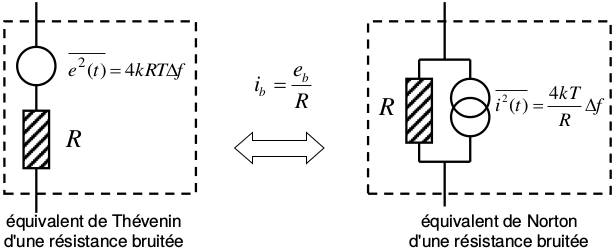
\includegraphics[width=0.8\textwidth,height=10\baselineskip,keepaspectratio]{ch3/image1} 
	\caption{Bruit thermique dans une résistance}
	\label{fig:bruitresist}
\end{figure}
\paragraph{Dans un transistor:} rappelons qu'un amplificateur différentiel est constitué de transistors. Les sources de bruits sont:
\begin{itemize}
	\item bruit thermique des résistances vraies (\(R_{BB}'\))
	\item bruit de grenaille des courants (base et collecteur)
	\item bruit en 1/f du transistor
\end{itemize}
La modélisation du bruit est présenté à la \autoref{fig:bruittrans}.
\begin{figure}[H] 
	\centering 
	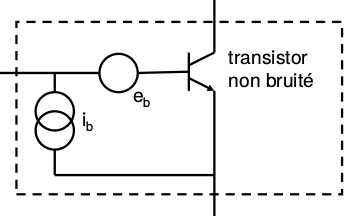
\includegraphics[width=0.4\textwidth,height=10\baselineskip,keepaspectratio]{ch3/image2} 
	\caption{Bruit dans un transistor}
	\label{fig:bruittrans}
\end{figure}
\paragraph{Dans un AOP:} rappelons qu'on AOP est constitué de résistances et de transistors. Le bruit est modélisé par la \autoref{fig:bruitaop}.
\begin{figure}[H] 
	\centering 
	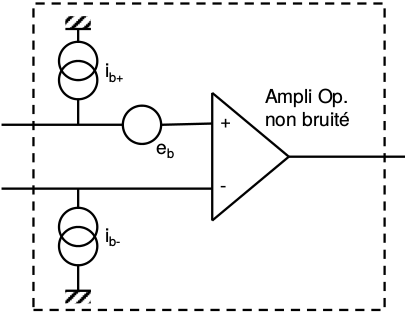
\includegraphics[width=0.8\textwidth,height=10\baselineskip,keepaspectratio]{ch3/image3} 
	\caption{Bruit dans un amplificateur opérationnel} 
	\label{fig:bruitaop}
\end{figure}
\paragraph{Remarques:} Les courants \(i_{b^\pm} \neq\) courant de bias (= courant constant de polarisation). \(i_{b^\pm}\) sont des courants à moyenne nulle, allant vers le circuit et dont l'impact dépend de l'impédance (+ l'impédance est grande, + le bruit est grand).
\subsection{Limitation de bruit}
\subsubsection{Introduction et principales techniques}
Le but de cette sous-section est de développer des méthodes afin de rendre l'amplitude du bruit négligeable face à celle du signal, c-à-d \(\nearrow\) SNR. Pour ce faire, il est possible d'agir sur 2 choses:
\begin{enumerate}
	\item Augmenter le signal, c-à-d amplifier dès que possible et autant que possible le signal \(\Rightarrow\) pré-ampli à grand gain et faible bruit.
	\item Réduire le bruit de tous les composants.
\end{enumerate}
Afin de parvenir à un résultat, il est important de suivre ces quelques règles de base:
\begin{enumerate}
	\item Cibler le type de bruit (afin de choisir des contre-mesures efficaces).
	\item S'attaquer au bruit prépondérant (on va peut-être s'occuper du gros d'abord, non ?).
	\item S'attaquer au bruit dès que possible (chaque module apportant son propre bruit (irréversible), il devient impossible de séparer les bruits entre eux au fur et à mesure que l'on avance sur la chaîne)
\end{enumerate}
Nous pouvons agir:
\begin{description}
\item \emph{Au niveau des composants:}
\begin{itemize}
	\item Choisir des composants à faible bruit.
	\item Jouer sur les paramètres influençant directement le bruit (ex. réduire la température pour un bruit thermique).
\end{itemize}
\item \emph{Au niveau du système:}
\begin{itemize}
	\item \hyperref[subsubsec:entreenobruit]{Pré-ampli à faible bruit} (parfois étage à transistor discrets afin de minimiser le bruit de l'aop, lui-même constitué d'un nombre conséquent de transistors discrets).
	\item \nameref{subsubsec:bandepass} (réduire le bruit dans un bande passante plus restreinte).
	\item \nameref{subsubsec:résistsource}.
	\item \nameref{subsubsec:detectsync} pour le bruit rose.
\end{itemize}
\end{description}
\subsubsection{Réduire la bande passante} \label{subsubsec:bandepass}
Le bruit à virtuellement une bande passante infinie alors que celle du dispositif de mesure est limitée \(\Rightarrow\) bruit perçu limité à la bande passante du dispositif.\bigbreak

Pour un bruit blanc de densité \(e_{bb}\) perçu au travers d'une bande passante \(B=f_{\text{max}}-f_{\text{min}}\):
\begin{equation}
E_b^2 = \int_{f_{\text{min}}}^{f_{\text{max}}} dE_b^2 = \int_{f_{\text{min}}}^{f_{\text{max}}} e_{bb}^2\,df = e_{bb}^2(f_{\text{max}}-f_{\text{min}}) 
\end{equation}
Ainsi, la valeur efficace du bruit dans une bande de fréquence, permettant d'avoir une idée sur l'amplitude du bruit, est:
\begin{equation}\label{eq:valeffbruitDB}
E_b = e_{bb}\sqrt{B}
\end{equation}
On déduit de \eqref{eq:valeffbruitDB} que plus la bande passante du dispositif de mesure \(\nearrow\), plus le bruit présent à la sortie de la chaîne de mesure \(\nearrow\) et donc plus le signal est perturbé. \(\Rightarrow\) Il faut \textbf{limiter la bande passante} (filtrage).\bigbreak

Dans un dispositif réel, le bruit est un "bruit composite" (rose (aux basses fréquences) + blanc (aux hautes fréquences)). Le point où les 2 densités spectrales sont égales (rose \(\cup\) blanc) est appelé la \emph{fréquence coin}.
\begin{figure}[H]
	\centering
	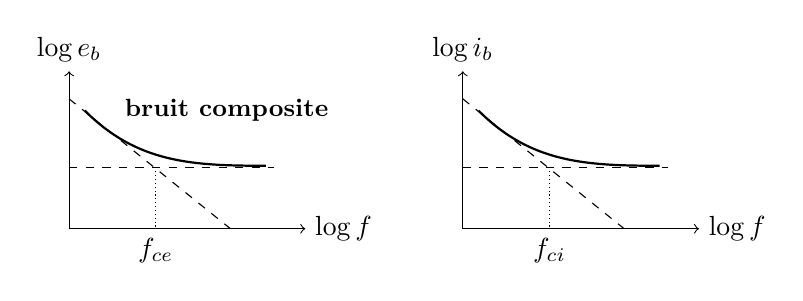
\begin{tikzpicture}
		\draw[dashed] (0,1.65) -- (2.05,0);
		\draw[dashed] (0,0.78) -- (2.6,0.78);
		\draw[densely dotted] (1.1,0.78) -- (1.1,0) node[below]{\(f_{ce}\)};
		\draw[thick] (0.2,1.5) to[out=-45, in=180] (2.5,0.8);
		\draw[->] (0,0) -- (0,2) node[above]{\(\log e_b\)};
		\draw[->] (0,0) -- (3,0) node[right]{\(\log f\)};
		\draw (2,1.5) node{\textbf{\small bruit composite}};
		\draw[dashed] (5,1.65) -- (7.05,0);
		\draw[dashed] (5,0.78) -- (7.6,0.78);
		\draw[densely dotted] (6.1,0.78) -- (6.1,0) node[below]{\(f_{ci}\)};
		\draw[thick] (5.2,1.5) to[out=-45, in=180] (7.5,0.8);
		\draw[->] (5,0) -- (5,2) node[above]{\(\log i_b\)};
		\draw[->] (5,0) -- (8,0) node[right]{\(\log f\)};
		\end{tikzpicture}
\end{figure}
La valeur efficace de bruit composite dans la bande passante est :
\begin{equation}
E_b^2 = e_{bb}^2\left[(f_{\text{max}}-f_{\text{min}})+f_{ce}\ln\left(\frac{f_{\text{max}}}{f_{\text{min}}}\right)\right]
\end{equation}
Ainsi, pour réduire le bruit il faut:
\begin{itemize}
	\item limiter la bande passante (\(f_{\text{max}}-f_{\text{min}}\))
	\item choisir des composants pour minimiser:
	\begin{itemize}
		\item la densité spectrale de bruit blanc \(e_{bb}\text{ (et }i_{bb}\))
		\item la fréquence de coupure \(f_{ce}\text{ (et }f_{ci}\))
	\end{itemize}
\end{itemize}
\subsubsection{Résistance de source} \label{subsubsec:résistsource}
\begin{description}
	\item[\(R_s\)] résistance de sortie du capteur (ou de l'étage précédent)
\end{description}
Un AOP comprend des sources de tension de bruit et de courant de bruit, il faut donc choisir un ampli à:
\begin{itemize}
	\item faible tension de bruit lorsque \(R_s\) est faible
	\item faible courant de bruit lorsque \(R_s\) est élevée
\end{itemize}
\subsubsection{Étage d'entrée à faible bruit} \label{subsubsec:entreenobruit}
Comparons 2 cas possible d'étage d'entrée de gain total \(G\):\bigbreak
\underline{Amplificateur unique:}  soit sa densité spectrale de bruit ramené à l'entrée \(v_b^{in}\), le bruit total à la sortie vaut
\begin{equation}\label{eq:etasortieunique}
v_b^{out}=G . v_b^{in}
\end{equation}
\underline{Ajout d'un étage d'entrée à faible bruit:} soit un 1\up{er} étage d'entrée de gain \(G_1\) et de densité spectrale de bruit (entrée) \(v_{b_1}^{in}\) et un 2\up{ème} étage de gain \(G_2\) et de densité spectrale de bruit (entrée) \(v_{b_2}^{in}\) tel que \(G_1 . G_2 = G\). Nous aurons donc à la sortie du premier étage:
\begin{itemize}
	\item le bruit dû au 1\up{er} étage: \(v_{b_1}^{out}=G_1 . v_{b_1}^{in}\)
	\item le bruit dû au 2\up{ème} étage: \(v_{b_2}^{in}\)
\end{itemize}
Et donc, le bruit total à la sortie vaut:
\begin{equation}\label{eq:etasortie}
v_b^{out} = G_2\sqrt{\left(v_{b_1}^{out}\right)^2 + \left(v_{b_2}^{in}\right)^2} = G\sqrt{\left(v_{b_1}^{in}\right)^2 + \left(v_{b_2}^{in}/G_1\right)^2}
\end{equation}
On remarque que le bruit total de \eqref{eq:etasortie} sera plus faible que celui de \eqref{eq:etasortieunique} si \(G_1\gg 1\text{ et } v_{b_1}^{in}<v_b^{in}\)
\begin{center}
	\textbf{le bruit d'un ampli est minimisé en plaçant en tête un préamplificateur à faible bruit et de gain suffisant}
\end{center}
\subsubsection{Détection synchrone} \label{subsubsec:detectsync}
Si le signal utile se situe à basse fréquence, le bruit en 1/f (rose) domine \(\Rightarrow\) transposer momentanément le signal utile à une fréquence plus élevée, à l'aide d'une modulation d'amplitude (signal sera au alentour de la fréquence porteuse), afin de réaliser la transmission ou l'amplification en dehors de la bande bruitée. 
\begin{figure}[H] 
	\centering 
	\begin{tikzpicture}
	 	\draw plot[domain=0:3*pi] (\x,{0.6*sin(\x r)}) node[right]{signal};
	 	\draw plot[samples=300,domain=0:3*pi] (\x,{0.6*sin(20*\x r)*(1+0.6*sin(\x r)) -2}) node[right]{AM};
	 	\node[draw,ellipse] (C) at (-0.5,-4){capteur};
	 	\node[draw] (M) at (2.5,-4){modulation};
	 	\node[draw] (A) at (5,-4){ampli};
	 	\node[draw] (D) at (7.5,-4){démodulation};
	 	\node[draw] (P) at (10.5,-4){Passe-bas};
	 	\draw[->, >=latex'] (C) -- (M);
	 	\draw[->, >=latex'] (M) -- (A);
	 	\draw[->, >=latex'] (A) -- (D);
	 	\draw[->, >=latex'] (D) -- (P);
	\end{tikzpicture} 
	\caption{Détection synchrone} 
\end{figure}
Pour résumer:
\begin{itemize}
		\item {\makebox[4cm]{signal utile:\hfill} \(s(t)\)}
		\item {\makebox[4cm]{signal modulation:\hfill} \(u_{mod}(t)=\cos(2\pi f_ut)\)}
		\item {\makebox[4cm]{signal démodulation:\hfill} \(u_{demod}(t) = \cos(2\pi f_ut+\varphi)\)}
\end{itemize}\ \\
Et donc, le signal modulé vaut:
\begin{equation}
s_{mod}(t) = s(t) . u_{mod}(t)
\end{equation}
qui est bien transposé autour de la fréquence \(f_u\) (\(f_u\gg f_{max}\)). Pour démoduler, nous utilisons une démodulation synchrone, c-à-d en multipliant par la même sinusoïde que lors de la modulation (+ déphasage inévitable \(\varphi\))
\begin{equation}
\begin{split}
s_{demod}(t) &= s_{mod}(t) . u_{demod}(t)\\
&= s(t)\cos(2\pi f_u t)\cos(2\pi f_u t+\varphi)\\
&= s(t)\frac{1}{2}\{\underbrace{\cos\varphi}_{\cst}+\cos(4\pi f_u t+\varphi)\}
\end{split}
\end{equation}
qui, après un filtre passe-bas (\(f_c \approx f_{max}\)) devient:
\begin{equation}
s_{demod}'(t) = s(t)\frac{\cos\varphi}{2}
\end{equation}
\section{Les parasites}
\subsection{Introduction}
Les parasites sont des tensions ou courants indésirables, d'origine extérieure à l'appareil perturbé, se superposant au signal utile. Ceux-ci apparaissent par suite du couplage d'un circuit source avec le circuit perturbé (victime).\bigbreak

L'origine physique le plus courant de ces parasites sont les parasites électromagnétiques (expliqués par les équations de Maxwell). Toutes charges et courants génèrent des champs (\(E\) et \(H\) variables, formant une onde électromagnétique) qui se transforment en f.e.m. (\(\int E\) ou \(H\) loi de Lenz). Il existe néanmoins d'autres phénomènes physiques comme la thermoélectricité, la piézoélectricité, etc.\bigbreak

À cela se rajoute le concept de champ proche et champ lointain ainsi que le type de couplages (C.f \autoref{fig:champproloin} et \autoref{fig:typcouplage})
\begin{figure}[H] 
	\centering 
	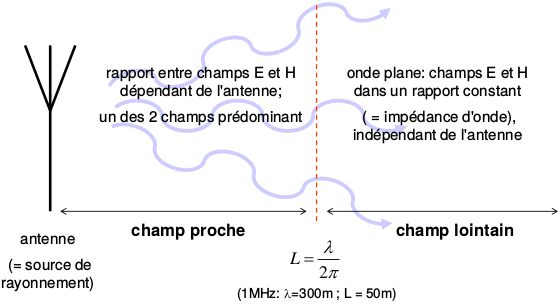
\includegraphics[width=0.8\textwidth,height=10\baselineskip,keepaspectratio]{ch3/image4} 
	\caption{Champ proche et champ lointain} 
	\label{fig:champproloin}
\end{figure}
\begin{figure}[H] 
	\centering 
	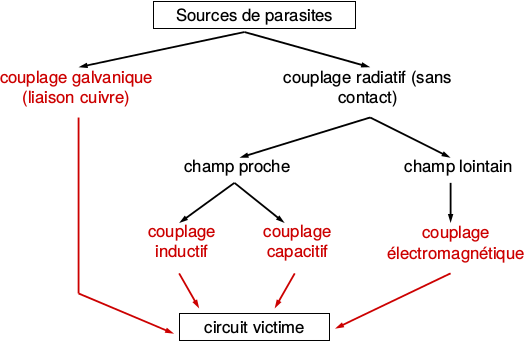
\includegraphics[width=0.8\textwidth,height=10\baselineskip,keepaspectratio]{ch3/image5} 
	\caption{Type de couplages}
	\label{fig:typcouplage} 
\end{figure}
Quelques exemples de parasites sont cités slide 46.
\subsection{Parasites rayonnés}
\subsubsection{Couplage capacitif}
Les charges portées par un conducteur induisent des charges opposées (\(\Rightarrow\) courant) dans un autre conducteur via le champ électrostatique \(E\). Existe entre toute paire de conducteurs et est modélisé par une capacité parasite entre ces conducteurs. À prendre en compte dans le domaine du \textbf{champ proche} (\(L<\lambda/2\pi\)). Ex.: pistes proches ou superposée dans les circuits imprimés, les bus, etc.\bigbreak

\(\Rightarrow\) éviter les lignes parallèles, éloigner le plus possible les fils les uns des autres afin de réduire les capacités parasites ou disposer d'un blindage électrostatique (décrit plus bas).

Un cas particulier existe, les \textbf{décharges électrostatiques}:
\begin{description}
	\item[définition] claquage de l'isolant entre les armatures du condensateur parasite lorsque le champs électrique devient trop important
	\item[exemple] tapis, vêtement en laine, éclair en cas d'orage, claquage de l'oxyde de grille dans les circuits MOS
	\item[contre-mesure] mise à la terre des dispositifs/utilisateurs pour les décharger et éviter l'accumulation de charge, intégrer un dispositifs de dissipation de puissance (parasurtenseurs, décrit plus bas)
\end{description}
Un exemple de dispositif permettant d'empêcher l'accumulation de charge se trouve \autoref{fig:dispdechdio}. La diode protectrice protège le circuit en aval en permettant le passage du courant parasite en cas de surtension.
\begin{figure}[H] 
	\centering 
	\begin{circuitikz}
	\draw (0,0) node[left]{\SI{0}{\volt}} to[short] (4,0) to[open] (4,1) to[short] (0,1) node[left]{\SI{5}{\volt}};
	\draw (2,0) to[sDo,l_=\SI{6}{\volt}] (2,1);
	\end{circuitikz}
	\caption{Dispositif de décharge} 
	\label{fig:dispdechdio}
\end{figure}
\subsubsection{Couplage inductif}
Un champ magnétique variable induit dans un conducteur une f.e.m. qui tend à s'opposer à cette variation (loi de Lenz). Existe en théorie dans toute paire de conducteur et est modélisé par une inductance mutuelle parasite entre ces conducteurs. À prendre en compte dans le domaine du \textbf{champ proche} (\(L<\lambda/2\pi\)). Ex.: lignes de signal (téléphone, instrumentation) entre elles ou placées à coté d'une ligne d'alimentation/moteur électrique etc.\bigbreak

Il faut donc éloigner les sources de champ magnétique, minimiser la surface offerte au champ magnétique extérieure (réduire l'inductance mutuelle en jouant sur l'orientation spatiale ou sur la surface de la boucle, en tressant les câbles par exemple), implémenter un blindage magnétique (décris plus bas).\\
Mode de couplage le plus répandu, toute boucle formée de conducteur est une victime potentielle. Phénomène d'autant plus critique que la fréquence est élevée. 

Un cas particulier, les \textbf{câbles de transmission}. Ceux-ci forment une boucle et sont donc des victimes privilégiés. Il existe quelques contre-mesures:
\begin{itemize}
	\item réduire la surface de la boucle:
	\begin{itemize}
		\item réduire la longueur des câbles
		\item rapprocher les conducteurs aller et retour
		\item torsader les fils d'amenée et de retour. Si au-delà des quelques \si{\mega\hertz}, passer au câble coaxial (mutuelle nulle).
	\end{itemize}
	\item câbles blindés
	\item passer à une transmission ayant une meilleur immunité:
	\begin{itemize}
		\item boucle de courant (si la transmission est en courant, il n'y a pas d'impact)
		\item porter l'information sur la fréquence
		\item passer au numérique
		\item code détecteurs/correcteurs d'erreur
	\end{itemize}
\end{itemize}

\subsubsection{Couplage électromagnétique}
Dans le domaine du \textbf{champ lointain} (\(L>\lambda/2\pi\)), \(E\) et \(H\) coexistent sous forme d'une onde plane. Tout conducteur peut se comporter comme une antenne réceptrice parasite à l'onde plane. C'est d'autant plus critique que la fréquence est élevée. Ex.: GSM dans les hôpitaux ou les avions etc.\bigbreak

Il faut donc limiter la source d'émission, implémenter un blindage EM (plus bas), designer le circuit récepteur, ou  utiliser un dispositif optique (comme la fibre optique).
\subsubsection{Blindage}
\underline{\textit{Blindage électrostatique} (champ proche)}: utiliser un matériau conducteur dont le potentiel est imposé. Ceci offre un chemin de retour pour le courant parasite et évite de modifier le potentiel du circuit victime. Le plus souvent, c'est une mise à la terre via une impédance faible. Ex.: blindage complet (boîtier) ou \autoref{fig:blindelectrostat}.\\
Il faut bien comprendre ici qu'au lieu de réduire la capacité parasite, nous interposons des conducteurs supplémentaires dont le potentiel est fixé. De plus, rien ne nous interdit de fixer un potentiel différent de la masse/terre (\SI{0}{\volt})
\begin{figure}[H] 
	\centering 
	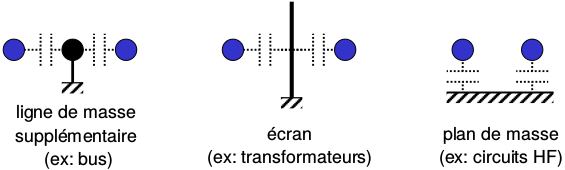
\includegraphics[width=0.7\textwidth,height=10\baselineskip,keepaspectratio]{ch3/image6} 
	\caption{Forme de blindage électrostatique}
	\label{fig:blindelectrostat}
\end{figure}
\begin{figure}[H] 
	\centering 
	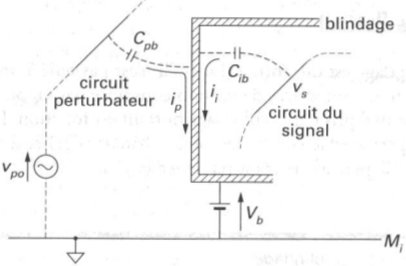
\includegraphics[width=0.8\textwidth,height=10\baselineskip,keepaspectratio]{ch3/image7} 
	\caption{Blindage électrostatique}
\end{figure}
\underline{\textit{Blindage magnétique} (champ proche)}: ici nous avons 2 cas:
\begin{itemize}
	\item champ BF: matériau ferromagnétique (\(\mu\) élevé). Il dévie les lignes de champ magnétique, mais il faut faire attention à la saturation \(\Rightarrow\) grande épaisseur du ferromagnétique (mais cher et lourd) (\autoref{fig:blindmagn}).
	\item champ HF: matériau conducteur (non ferromagnétique). les courants de Foucault induits dans le blindage s'opposent à la pénétration du champ extérieur.
\end{itemize}
\begin{figure}[H] 
	\centering 
	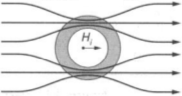
\includegraphics[height=4\baselineskip]{ch3/image8} 
	\caption{Blindage ferromagnétique}
	\label{fig:blindmagn}
\end{figure}

\underline{\textit{Blindage EM} (champ lointain)}: utiliser un matériau conducteur qui supprimera le champ perturbateur par un champ opposé induit (courant de Foucault). Typiquement, une cage de Faraday. Néanmoins, il nécessite de faire rentrer les lignes de signal et d'alimentation (coucou couplage inductif) et la moindre ouverture réduit l'efficacité du blindage \(\Rightarrow\) construction très délicate.\bigbreak

\underline{\textit{Remarques générales}}: Les blindages concerne tout autant les câbles de transmission que les boîtiers (capteur, instrumentation). De plus la connections des blindages de câbles n'est pas trivial.
\subsection{Parasites conduits}
\subsubsection{Introduction}
Commençons pas définir ce qu'est un \emph{couplage galvanique}:
\begin{description}
	\item[définition] transmission d'un signal perturbateur entre la source de ce signal et le dispositif victime \emph{via un conducteur commun}.
\end{description}
Ceci concerne autant les lignes de signal que les alims/masse/terre et le simple fait de brancher 2 appareils sur le réseau électrique établit un couplage galvanique. Comme par exemple 2 appareils à \SI{220}{\volt} dans 2 pièces différentes, connectés à la masse. Si l'un demande en puissance, cela fait baisser la tension dans tout le circuit. Il existe 2 origines distinctes:
\begin{enumerate}
	\item le conducteur commun (idéal) transmet un signal parasite issu d'un autre équipement (comme parasite transmis via les lignes d'alimentation à cause de la foudre).
	\item le conducteur commun n'est pas équipotentiel \(\Rightarrow\) la circulation d'un courant sur ce conducteur génère des f.e.m. parasites.
\end{enumerate}
Ces 2 origines sont bien évidement cumulables. Il existe 2 niveaux de conséquences:
\begin{enumerate}
	\item dégrade le signal (superposition du signal utile et parasite, si sur alim \(\rightarrow\) mauvais fonctionnement du circuit).
	\item détruit l'équipement (surtension (claquage électrostatique) ou surpuissance (destruction par échauffement)).
\end{enumerate}
Remarquons que tout parasite rayonné devient f.e.m. ou courant sur un conducteur et donc que les conséquences sont aussi valables pour les parasites rayonnés en amont.
\subsubsection{Contre-mesures}
Il existe 3 contre-mesures générales:
\begin{enumerate}
	\item Contre les parasites conduits issus d'autres équipement:
	\begin{itemize}
		\item filtre passe-bas pour le spectre étendu, filtre réjecteur de fréquence pour le spectre étroit
		\item équilibrer (rendre le circuit plus symétrique, voir plus bas)
	\end{itemize}
 \hspace*{\dimexpr\linewidth-\textwidth\relax}%
 \begin{minipage}[t]{\textwidth}%
 	Néanmoins, il n'est pas trivial de réaliser le filtre, nous pouvons utiliser un filtre passif (capa et inductance) ou actif (passif + AOP), en mode commun ou différentiel.
 \end{minipage} 
	\item Contre les parasites générés par l'impédance des connexions:
	\begin{itemize}
		\item design des connexions (\(\searrow\) longueur + \(\nearrow\) section conductrice \(= \searrow\) impédance)
		\item connecter judicieusement les alimentations et les masses:
		\begin{enumerate}
			\item éviter les chemins communs \(\Rightarrow\) câblages en étoile
			\item séparer alimentations de signaux à fréquence et/ou puissance \(\neq\)
		\end{enumerate}	
	\end{itemize}
	\item Contre la destruction des équipement par surtension/surpuissance \(\Rightarrow\) parasurtenseurs, dont le principe est de limiter la tension  et ayant la capacité de dissiper l'énergie excédentaire:
	\begin{itemize}
		\item diodes Zener utilisée en avalanche (protection)
		\item varistance (résistance non linéaire, \(\nearrow\) tension \(= \searrow\) résistance)
		\item éclateurs (tube à gaz dissipant temporairement l'énergie via un arc électrique)
	\end{itemize}
\end{enumerate}
\underline{\textit{Exemple} (flemme)}:
\begin{figure}[H] 
	\centering 
	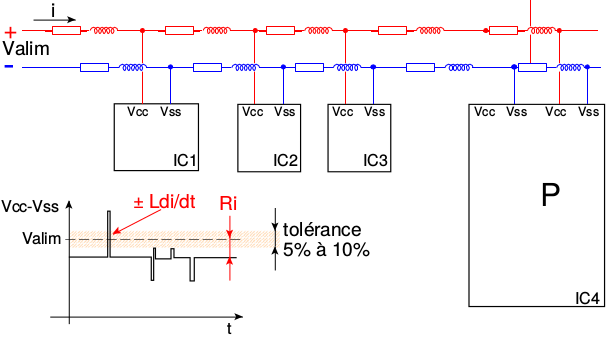
\includegraphics[width=0.8\textwidth,height=10\baselineskip,keepaspectratio]{ch3/image9} 
	\caption{Circuit électronique initial} 
\end{figure}
A première vue, les fils ou pistes d'alimentation sont des équipotentielles. En réalité, il existe souvent une distance de plusieurs centimètres ou dizaines de centimètres entre les bornes d'alimentation d'une carte électronique et le circuit intégré le plus éloigné.\\
L'impédance de ces connections joue un rôle non négligeable:
\begin{itemize}
\item la chute de tension ohmique due à la résistance des connections (l'épaisseur des piste est très faible: de l'ordre de \SI{30}{\micro\meter}) parcourue par le courant moyen.
\item les fluctuations de tension liées aux variations de courant importantes (basculement de portes, charge de capacités parasites, "réveil" d'un circuit CMOS) sur l'inductance des connections \(\rightarrow\) peuvent faire sortir l'alimentation de sa plage normale.
\end{itemize}
\begin{figure}[H] 
	\centering 
	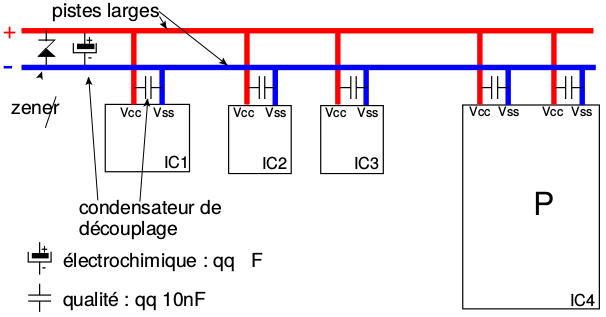
\includegraphics[width=0.8\textwidth,height=10\baselineskip,keepaspectratio]{ch3/image10} 
	\caption{Circuit électronique final} 
\end{figure}
Les améliorations les plus courantes de l'alimentation sont
\begin{itemize}
\item l'utilisation de fils de plus forte section ou de pistes plus larges (quelques \si{\milli\meter}) ou de circuits multi-couches (permettant d'inclure plan de masse et plan d'alimentation)
\item les condensateurs de découplage sous forme
\begin{itemize}
	\item d'un condensateur électrolytique (généralement quelques \si{\micro\farad}) 
	\item d'un ensemble de condensateurs de très bonne qualité disséminés sur toute la carte, le plus près possible des pattes d'alimentation de chaque gros circuit intégré et de chaque groupe de petits circuits

\end{itemize}
\item une diode Zener (protection contre les surtensions)
\end{itemize}
Les condensateurs constituent des sources de tension localisée (à très court terme) vis-à-vis des impulsions de courant consommées par les circuits intégrés.\bigbreak

Le mot "découplage" qualifie le fait que les variations de consommation (composante alternative) propres du circuit ne sont pas vues par les fils d'alimentation, qui ne véhiculent que la composante continue (moyenne). Les inductances parasites du câblage ont donc beaucoup moins d'influence.\bigbreak

La diode Zener permet d'écrêter les surtensions transitoires. Si celles-ci sont répétitives, l'absorption d'énergie par la Zener peut excéder ses capacités de refroidissement et la détruire. En cas de tension d'entrée trop importante, la Zener va également surchauffer et fondre, généralement en court-circuit, ce qui protégera les circuits coûteux en aval.
\subsubsection{Isolation galvanique}
\begin{description}
	\item[définition] coupure de tout lien galvanique entre 2 parties du montage
	\item[moyen] couplage magnétique (transformateur) et couplage optique (optocoupleur, fibre optique)
\end{description}
C'est souvent nécessaire pour des raisons de protection des utilisateurs et des équipements (sécurité). Le but est de faire passer de la puissance/info d'une autre manière que via de l'électricité.
\iffalse \subsection{Compatibilité électromagnétique}
\begin{description}
	\item[définition] discipline ayant pour but d'analyser et de résoudre l'ensemble des problèmes de parasitage EM d'un équipement par un autre
\end{description}
C'est une discipline de plus en plus importante en raison de la multiplications des équipement électroniques. Il existe des normes stricte depuis les années 90. On définit:
\begin{description}
	\item[CEM/EMC] compatibilité EM
	\item[IEM/EMI] interférence EM
\end{description}
\subsection{Notions embrassées par la CEM}
les normes CEM, les types de couplages, les imperfections des composants (passif et surtout actifs car sources de perturbations), les boîtiers et blindages, le câblage, le routage des pistes dans les circuits imprimés (surtout masse et alim) et « tous les effets du second ordre ».
\subsection{Exemple: alimentation à découpage}
Exemple slide 81--85.\fi
\section{Câblage et connexions}
\subsection{Référence d'un signal}
Rappel sur tension et masse slide 88. Nous ajoutons quelques subtilités:
\begin{enumerate}
	\item impédance de masse: en pratique la "masse" d'un montage peut être un conducteur ayant une certaine extension physique \(\Rightarrow\) impédance \(\neq 0 \Rightarrow\) lorsque parcouru par un courant, pas équipotentiel \(\Rightarrow\) plus vraiment une masse (f.e.m. parasite)
	\item plusieurs montages: les masses de différents montages sont à priori pas au même potentiel (pas connecté ou connecté via des impédance \(\neq 0\))
\end{enumerate}
Pour rappel, la mise à terre est une connexion d'un conducteur au potentiel de la terre (sol) afin d'assurer la protection des utilisateurs et des équipements (le réseau de terre doit avoir l'impédance la plus faible possible). La masse (référence) et la terre (protection) ne sont pas forcément connectées.\bigbreak

On définit les appareils:
\begin{description}
	\item[flottants] aucune des 2 bornes du signal (entrée ou sortie) n'est connectée à la terre (appareils portatifs, appareils sur réseau à 3 bornes)
	\item[non flottants] masse = terre
\end{description}
\subsection{Montage "single-ended"}
\subsubsection{Cas idéal}
Un montage "single-ended" possèdent les caractéristiques suivantes:
\begin{itemize}
\item un amplificateur "single-ended" (= asymétrique) comme un (non-)inverseur, suiveur à AOP. Au niveau multiplexage, il faut \(N+1\) fils pour \(N\) signaux. \item La référence du capteur = la référence de l'instrumentation
\end{itemize} 
Dans le cas théorique \(V_{in}=e_s\) (donc pas de parasites).
\begin{figure}[H] 
	\centering 
	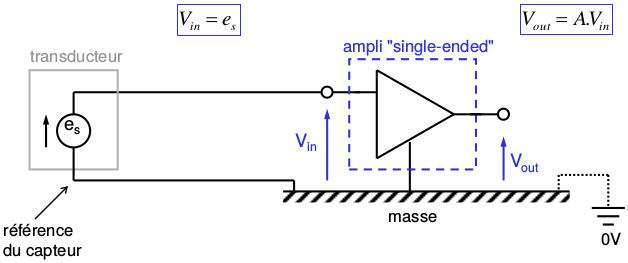
\includegraphics[width=0.8\textwidth,height=10\baselineskip,keepaspectratio]{ch3/image11} 
	\caption{Single-ended (idéal)} 
\end{figure}
\subsubsection{Cas réel}
Dans le cas réel, une source parasite \(e_p\) vient s'ajouter car il existe une impédance de masse non négligeable et des parasites induits dans la boucle. Il en résulte \(V_{in} = e_s + e_p\) et donc un signal dégradé.
\begin{figure}[H]
	\centering 
	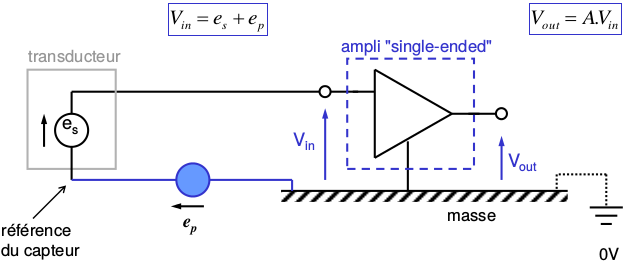
\includegraphics[width=0.8\textwidth,height=10\baselineskip,keepaspectratio]{ch3/image12} 
	\caption{Single-ended (réel)} 
\end{figure}
\(\Rightarrow\) éviter les montages "single-ended". Sauf si la chute de tension sur l'impédance de masse ET les f.e.m induites sont négligeables, comme pour:
\begin{itemize}
	\item un capteur proche de l'ampli
	\item un capteur éloigné mais isolé de son environnement et sa masse est ramenée à l'ampli par une connexion d'impédance négligeable
\end{itemize}
\subsection{Montage différentiel}
\begin{figure}[H] 
	\centering 
	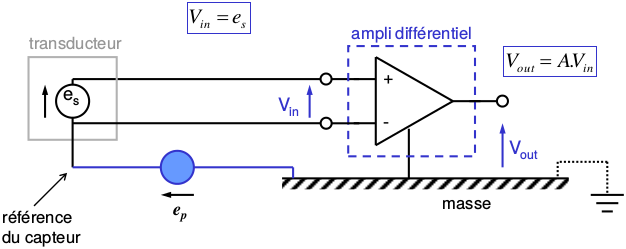
\includegraphics[width=0.8\textwidth,height=10\baselineskip,keepaspectratio]{ch3/image13} 
	\caption{Montage différentiel} 
\end{figure}
Dans ce montage, nous avons:
\begin{itemize}
		\item {\makebox[8cm]{tension d'entrée de l'ampli différentiel\hfill} \(V^-=e_p\qquad V^+=e_s+e_p\)} 
		\item {\makebox[8cm]{tension différentielle\hfill} \(V_{md} = V^+-V^-=e_s\)} 
		\item {\makebox[8cm]{tension de mode commun (parasites)\hfill} \(V_{mc}=\frac{V^++V^-}{2}=e_p+\frac{e_s}{2}\)} 
		\item {\makebox[8cm]{tension de sortie\hfill} \(V_{out}=A_{md}V_{md}+A_{mc}V_{mc}\)} 
		\item {\makebox[8cm]{taux de réjection en mode commum\hfill} \(\text{CMRR} = \frac{A_{md}}{A_{mc}}\)} 
\end{itemize}
Il faut donc maximiser le CMRR (common mode rejection ratio). On en déduit les avantages et inconvénients suivants:
\begin{description}
	\item[avantages]:
	\begin{itemize}
		\item les parasites de mode commun, les parasites par couplage galvanique et les autres parasites induits en mode commun sont rejetés
		\item signal dont aucune des bornes ne peut être considérée comme une masse (même imparfaite). ex: tension de déséquilibre d'un pont de Wheatstone ou un montage porté à une tension élevée.
	\end{itemize}
	\item [inconvénients]:
	\begin{itemize}
		\item les parasites de mode différentiel sont toujours amplifiés
		\item liaison \(2N\) (ou \(2N+1\)) fils pour \(N\) signaux
	\end{itemize}
\end{description}
\underline{\textit{Remarques}}: en instrumentation, la tension de mode commun est souvent du même ordre de grandeur  voir plus élevée que la tension différentielle. On essayera de faire apparaître les parasites sous forme de tension en mode commun car elles seront rejetés (pas entièrement, dépend du CMRR). Hélas, un bon CMRR ne suffit pas.
\begin{figure}[H] 
	\centering 
	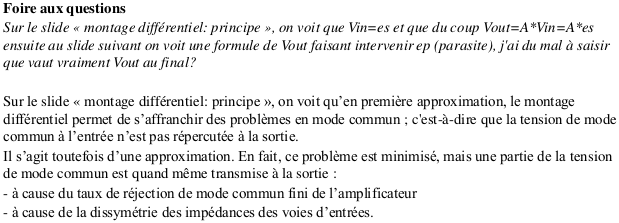
\includegraphics[width=0.8\textwidth,height=10\baselineskip,keepaspectratio]{ch3/image14} 
\end{figure}
Pour un multiplexeur, les deux montages s'implémentent comme illustré à la \autoref{fig:multmont}
\begin{figure}[H]
	\centering
	\subfigure[Single-ended]{\label{fig:multsing}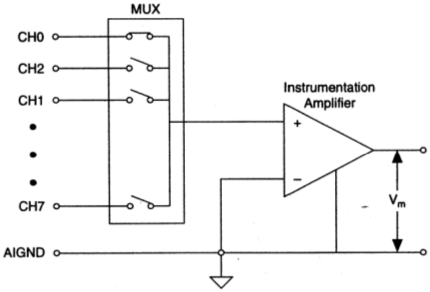
\includegraphics[width=0.4\textwidth]{ch3/image15}}
	\subfigure[Différentiel]{\label{fig:mutldiff}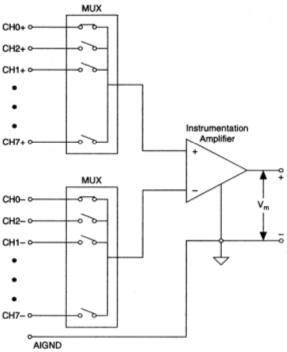
\includegraphics[height=15\baselineskip]{ch3/image16}}
	\caption{Implémentation avec un multiplexeur}
	\label{fig:multmont}
\end{figure}
\subsection{Symétrie des voies d'amenée}
\subsubsection{Déséquilibre série}
\begin{figure}[H] 
	\centering 
	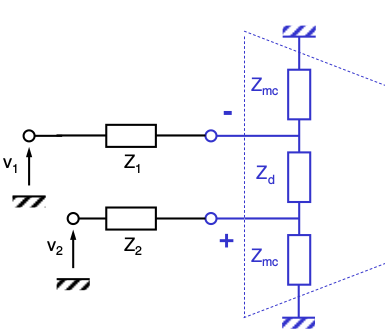
\includegraphics[width=0.8\textwidth,height=10\baselineskip,keepaspectratio]{ch3/image17} 
	\caption{Déséquilibre série} 
\end{figure}
Soit \(Z_1, Z_2\) les impédances série des voies d'amenée (souvent résistif) et soit un ampli différentiel ayant comme impédances d'entrée:
\begin{itemize}
	\item 1 impédance différentielle \(Z_d\) (hyp: \(\infty\))
	\item 2 impédances mode commun \(Z_{mc}\) (hyp: identiques)
\end{itemize}
Souvent \(Z_{mc} = \SI{e10}{\ohm}\)  \(\parallelsum\) capa en \si{\pico\farad} \(\Rightarrow \text{ passe-bas }f_c\approx \SI{10}{\hertz}\). Nous avons donc:
\[v_d = v_2-v_1\qquad v_d'=v^+-v^-\qquad v_{mc}=\frac{v_1+v_2}{2}\qquad v_{mc}'=\frac{v^++v^-}{2}\]
Les tensions à l'entrée de l'ampli sont:
\[v^-=\frac{Z_{mc}}{Z_1+Z_{mc}}v_1\qquad v^+=\frac{Z_{mc}}{Z_2+Z_{mc}}v_2\]
en faisant l'hypothèse que \(Z_{mc}\gg Z_1, Z_2\):
\[v_{mc}'\approx v_{mc}\qquad v_d'=v_d+\frac{Z_1-Z_2}{Z_{mc}}v_{mc}\]
La tension différentielle est polluée par une fraction de la tension de mode commun, fraction d'autant plus importante que \(Z_1\text{ et }Z_2\) sont \(\neq\) et que \(Z_{mc}\) est petit. Tout déséquilibre engendrera une dégradation du CMRR. En particulier, il faut que \(R_1=R_2\) pour une bonne réjection des tensions de mode commun continues et basse fréquence.
\subsubsection{Déséquilibre parallèle}
\begin{figure}[H] 
	\centering 
	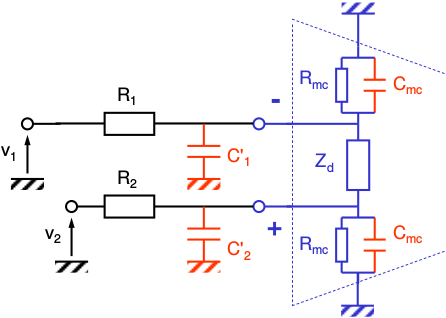
\includegraphics[width=0.8\textwidth,height=10\baselineskip,keepaspectratio]{ch3/image18} 
	\caption{Désiquilibre parallèle} 
\end{figure}
On ajoute maintenant \(C_1', C_2'\) des capa parasites \(\parallelsum\) venant s'ajouter aux 2 capas \(C_{mc}\) de l'ampli. Nous avons donc:
\[C_1=C_1'+C_{mc}\qquad C_2=C_2'+C_{mc}\] 
\begin{figure}[H] 
	\centering 
	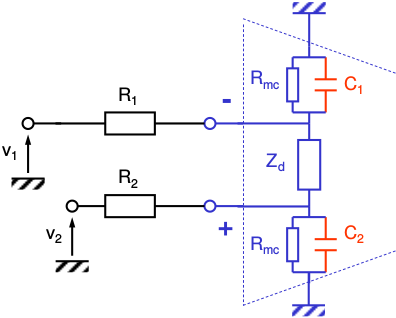
\includegraphics[width=0.8\textwidth,height=10\baselineskip,keepaspectratio]{ch3/image19}
\end{figure}
En supposant toujours que \(Z_d\gg\)
\[v^-=\frac{(R_{mc} \parallelsum C_1)}{R_1+(R_{mc} \parallelsum C_1)}\qquad v^+=\frac{(R_{mc} \parallelsum C_2)}{R_2+(R_{mc} \parallelsum C_2)}\] 
Dans la gamme de fréquence \(\frac{1}{R_{mc}C_1},\frac{1}{R_{mc}C_2}\ll\omega_{mc}\ll\frac{1}{R_1C_1},\frac{1}{R_2C_2}\) on a:
\[v_{mc}'\approx v_{mc}\qquad v_d'=v_d+j\omega(R_1C_1-R_2C_2)v_{mc}\]
La tension différentielle est polluée par une fraction de la tension de mode commun, fraction d'autant plus importante que \(C_1\text{ et }C_2\) sont différentes, mais cette fois, c'est surtout pour les fréquences plus élevées.\bigbreak

En pratique, \(C_1'\text{ et }C_2'\) sont des capas parasites qui existent vis-à-vis du blindage électrostatique des voies d'amenée, alors que précédemment, on a fait l'hypothèse d'être à la masse. En portant le blindage à la tension de mode commun \(v_{mc}\), on annule la tension différentielle parasite due au déséquilibre de \(C_1', C_2'\), c'est la \emph{garde}.
\begin{figure}[H] 
	\centering 
	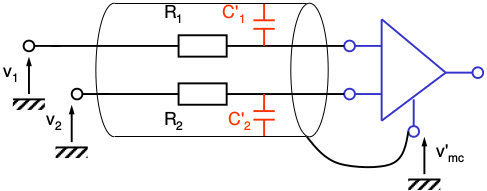
\includegraphics[width=0.7\textwidth,height=10\baselineskip,keepaspectratio]{ch3/image20} 
	\caption{Désiquilibre parallèle: garde} 
\end{figure}
\subsection{Montage différentiel avec \texorpdfstring{\(v_{mc}\)}{tension de mode commun} élevée}\label{subsec:montdiffvmcgrand}
Avant, on avait \(2N+1\) conducteurs et un \(v_{mc}\) relativement faible (les 2 références restaient proches). Dans le cas d'un source flottante (pas connectée à la référence) on a:
\begin{itemize}
	\item \(2N\) conducteurs
	\item tension de mode commun quelconque et variable dans le temps (AC + DC)
\end{itemize}
Une très mauvaise idée car nous avons une source de perturbations importante qui risque de détruite le matériel par surtension.

N.B.: vérifier la capa de l'ampli à tenir la tension de mode commun (\!?).
\subsubsection{1\up{ère} solution: bias resistor pour source flottante}
Il faut limiter la tension de mode commun, donc soit on utilise \(2N+1\) conducteurs (donc retour au cas précédent) soit on utilise des résistances offrant une liaison galvanique de haute impédance ("bias resistor):
\begin{itemize}
	\item meilleur symétrie que \(2N+1\) conducteurs
	\item valeur suffisamment élevée pour ne pas imposer le potentiel des entrées
	\item mais suffisamment faible pour éviter que la tension de mode commun soit trop éloignée de la référence de l’instrumentation
	\item typiquement: \SI{10}{\kilo\ohm} à \SI{100}{\kilo\ohm}
\end{itemize}
\begin{figure}[H] 
	\centering 
	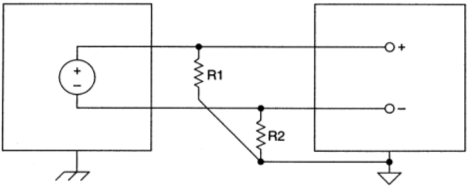
\includegraphics[width=0.7\textwidth,height=10\baselineskip,keepaspectratio]{ch3/image21} 
	\caption{bias resistor pour source flottante} 
\end{figure}
\subsubsection{2\up{ème} solution: ampli d'isolation}
\begin{figure}[H] 
	\centering 
	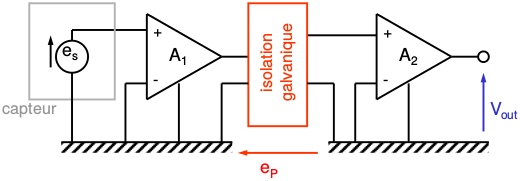
\includegraphics[width=0.7\textwidth,height=10\baselineskip,keepaspectratio]{ch3/image22} 
	\caption{Ampli d'isolation} 
\end{figure}
Comme ceci l'instrumentation au potentiel du capteur possède sa propre alimentation et donc pas de mode commun.
\subsection{Conclusion}
Il y a 3 cas à distinguer:
\begin{enumerate}
	\item les références sont identiques:
	\begin{itemize}
		\item différence de potentiel nulle ou négligeable: c'est l'exception, les f.e.m. par impédance de masse et parasites sont négligeables, la référence est indifféremment la masse ou la terre. Un simple montage asymétrique convient.
	\end{itemize}
	\item les références sont proches:
	\begin{itemize}
		\item tension de mode commun "faible": typiquement un cas \(2N+1\) fils. Un montage différentiel "simple" convient (il faut vérifier la limite de l'ampli vis-à-vis du mode commun)
	\end{itemize}
	\item les références sont éloignées:
	\begin{itemize}
		\item tension de mode commun élevée (ou quelconque): capteur flottant et porté à un potentiel élevé. Il faut limiter le mode commun \(\Rightarrow 2N+1\) fil ou bias resistors ou reprendre le mode commun grâce à l'ampli d'isolation.
	\end{itemize}
\end{enumerate}
De plus, au niveau de la boucle différentielle, les mesures classiques pour limiter les parasites sont le câble torsadé ou coaxial, le blindage des câbles (complexe), etc.
\section{Transmission des signaux}
\subsection{Introduction}
La majorité des transmissions des signaux se font par tension analogique, le montage différentiel ne résout pas tout (il résout surtout le couplage galvanique). Pour les environnements très parasités et/ou longues distances, nous aurons recours à des transmissions par boucle de courant, par fréquence, par signal optique ou des transmission numérique.
\subsubsection{Inconvénients d'une transmission en tension}
Illustrons une transmission en tension (\autoref{fig:transmtension}). Nous aurons donc \(R_{in}\) élevé et \(R_{out}\) faible (adaptation d'impédance en tension) mais la liaison à distance possède une \(R_{\text{fils}}\) non négligeable. La sortie obtenue est donc 
\[v = e\frac{R_{in}}{R_{out}+R_{in}+R_{\text{fils}}}<e\]
On a donc un affaiblissement du signal, 1\up{er} inconvénient.\\
Prenons le cas maintenant d'une tension parasite par couplage magnétique (\autoref{fig:transmtensionpara})
\[v = (e_s+e_p)\frac{R_{in}}{R_{out}+R_{in}}\]
Le parasite induit se superpose au signal, 2\up{ème} inconvénient
\begin{figure}[H] 
	\centering 
	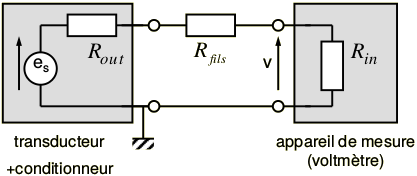
\includegraphics[width=0.6\textwidth,height=10\baselineskip,keepaspectratio]{ch3/image23} 
	\caption{Transmission en tension: résistance de ligne} 
	\label{fig:transmtension}
\end{figure}
\begin{figure}[H] 
	\centering 
	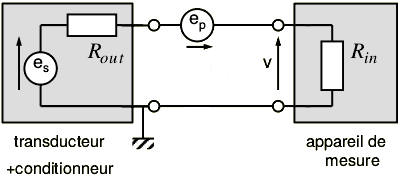
\includegraphics[width=0.6\textwidth,height=10\baselineskip,keepaspectratio]{ch3/image24} 
	\caption{Transmission en tension: parasite de ligne par couplage magnétique} 
	\label{fig:transmtensionpara}
\end{figure}
\subsection{Boucle de courant}
Le but est de passer l'information non plus par une tension, mais par un courant. Il est en pratique plus facile d'obtenir \(R_{out}\) (commande en courant) élevée que \(R_{in}\) élevée (commande en tension). Dans le cas de la \autoref{fig:transcourant}, nous obtenons \((R_{in}+R_{fils})i = R_{out}(i_s-i)\) et donc
\[i=\frac{R_{out}}{R_{out}+R_{in}+R_{fils}}i_s\]
L'affaiblissement du signal est beaucoup plus faible qu'en tension (car plus facile d'obtenir un \(R_{out}\) élevée qu'un \(R_{in}\) élevée).\\
Avec le couplage magnétique (\autoref{fig:transcourantpara}):
\[i_p=\frac{e_p}{R_{out}+R_{in}}\]
Comme \(R_{out}\) élevée, \(i_p\ll i_s \Rightarrow\) bonne immunité aux parasites magnétiques.\\
Plusieurs avantages:
\begin{itemize}
	\item bien pour transmission longue distance (\SI{1}{\kilo\meter} ou plus) car l'impédance des fils influence peu le courant
	\item bonne immunité aux f.e.m. induites car les valeurs idéales de \(R_{out}\text{ et }R_{in}\) sont plus facile à approcher en commande en courant qu'en commande en tension
	\item On peut utiliser un courant \(\neq0\) pour représenter la valeur 0 afin de détecter la rupture de la liaison
\end{itemize}
\begin{figure}[H] 
	\centering 
	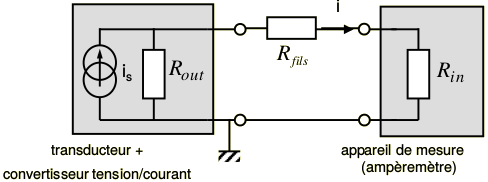
\includegraphics[width=0.6\textwidth,height=10\baselineskip,keepaspectratio]{ch3/image35} 
	\caption{Transmission en courant: résistance de ligne} 
	\label{fig:transcourant}
\end{figure}
\begin{figure}[H] 
	\centering 
	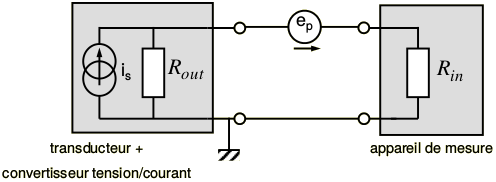
\includegraphics[width=0.6\textwidth,height=10\baselineskip,keepaspectratio]{ch3/image36} 
	\caption{Transmission en courant: parasite de ligne par couplage magnétique} 
	\label{fig:transcourantpara}
\end{figure}
\section{Câblage de la masse}
On a plusieurs circuits qui partagent la même alimentation et qui doivent s'échanger de l'information, chacun devant être connecté à une référence unique (masse). Comment câbler?
\subsection{Interconnexion des circuits}
Il faut éviter les impédances communes \(\rightarrow\) mettre en étoile \(\rightarrow\) si le PCM à une impédance nulle \(\Rightarrow\) pas de couplage d'impédance
\begin{figure}[H] 
	\centering 
	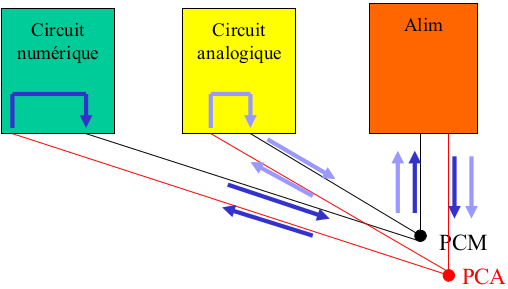
\includegraphics[width=0.8\textwidth,height=10\baselineskip,keepaspectratio]{ch3/image25} 
	\caption{Interconnexion des circuits en étoile} 
\end{figure} 
\subsection{Câblage de la masse analogique}
\begin{figure}[H] 
	\centering 
	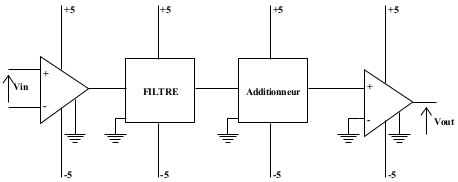
\includegraphics[width=0.6\textwidth,height=10\baselineskip,keepaspectratio]{ch3/image26}
\end{figure}
Dans le cas analogique, que faire ? Étoile ou cascade ?
\subsubsection{Masse en étoile}
\begin{figure}[H] 
	\centering 
	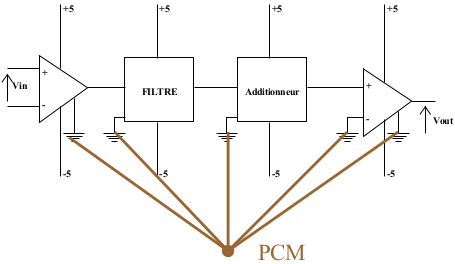
\includegraphics[width=0.8\textwidth,height=10\baselineskip,keepaspectratio]{ch3/image27} 
	\caption{Masse analogique en étoile} 
\end{figure}
\begin{description}
	\item[Avantages] pas d'impédance commune
	\item[Désavantages] longueur des pistes et formation de boucle
\end{description}
\subsubsection{Masse en cascade}
\begin{figure}[H] 
	\centering 
	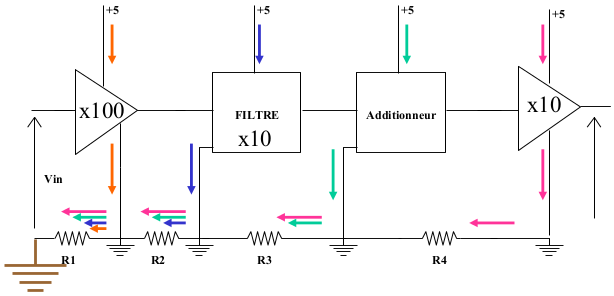
\includegraphics[width=0.8\textwidth,height=10\baselineskip,keepaspectratio]{ch3/image28} 
	\caption{Masse analogique en cascade (amont)} 
\end{figure}
Dans ce cas-ci, tous les courants passent pas \(R_1 \Rightarrow V_{in}=V_{out}/\num{e4}\) car on amplifie \(V_{in}+ i_iR_1\)!
\begin{figure}[H] 
	\centering 
	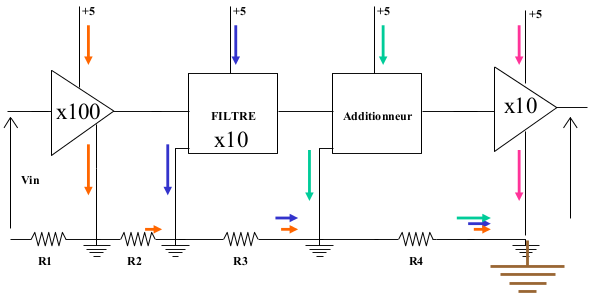
\includegraphics[width=0.8\textwidth,height=10\baselineskip,keepaspectratio]{ch3/image29} 
	\caption{Masse analogique en cascade (aval)} 
\end{figure}
Dans ce cas-là, nous avons minimiser les courants dans \(R_1\).
\subsection{Câblage de la masse numérique}
À haute fréquence, l'effet selfique des câbles devient dominant \(\Rightarrow\) pistes à grande impédance et courants passent par capas parasites\(\Rightarrow\) \cancel{masse en étoile} plan de masse (minimise les inductances et les boucles). Le courant suivra le chemin de moindre impédance.
\begin{figure}[H] 
	\centering 
	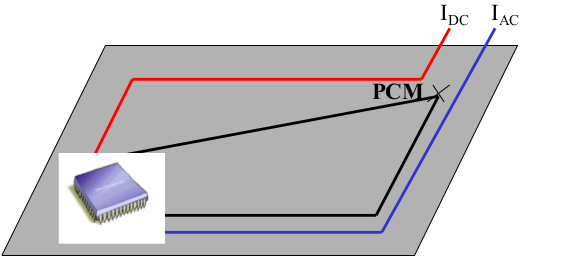
\includegraphics[width=0.5\textwidth,height=10\baselineskip,keepaspectratio]{ch3/image30} 
	\caption{Plan de masse} 
\end{figure}
\subsection{CAN et CNA}
\begin{figure}[H] 
	\centering 
	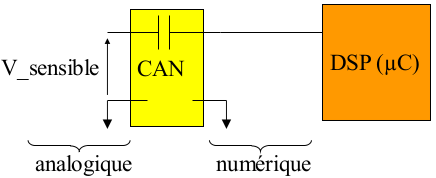
\includegraphics[width=0.5\textwidth]{ch3/image31} 
\end{figure}
Dans un CAN/CNA, il y a un faible courant qui circule à travers sa capa parasite.\\
Il faut 2 masses distinctes pour conserver une topologie en étoile et il faut placer le CAN sur le point central de masse
\begin{figure}[H] 
	\centering 
	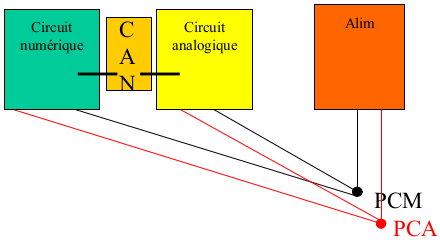
\includegraphics[width=0.7\textwidth,height=10\baselineskip,keepaspectratio]{ch3/image32} 
\end{figure}
\subsubsection{Câblage des alimentation}
2 problèmes se posent:
\begin{itemize}
	\item Ripple des alimentation à découpage (fluctuation autour de la valeur consigne)
	\item Consommation des différents circuits
\end{itemize}
\begin{figure}[H] 
	\centering 
	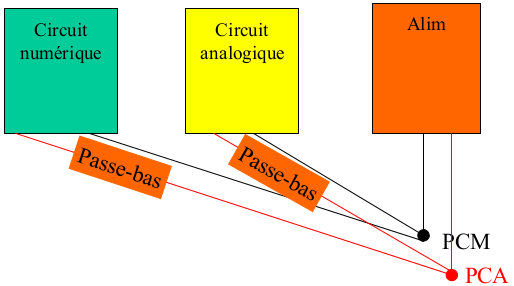
\includegraphics[width=0.7\textwidth,height=10\baselineskip,keepaspectratio]{ch3/image33}  
\end{figure}
Il faut mettre une capa a côté du composant, elle jouera le rôle de réservoir de charge. Sachant que la résistance parasite est d'autant plus grande que la capa est grande, on placera une plus petite capa en parallèle dans le cas HF car c'est la résistance qui est gênante.
\begin{figure}[H] 
	\centering 
	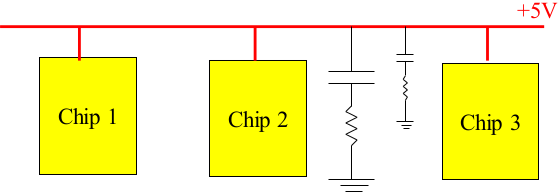
\includegraphics[width=0.6\textwidth,height=10\baselineskip,keepaspectratio]{ch3/image34}  
\end{figure}